%%%%%%%%%%%%
%
% $Autor: Wings $
% $Datum: 2019-03-05 08:03:15Z $
% $Pfad: Automatisierung/Skript/Produktspezifikation/Powerpoint/AMF.tex $
% $Version: 4250 $
%
%%%%%%%%%%%%

%Quelle:     \href{https://www.clickworker.de/2019/05/14/realistische-trainingsdaten-fuer-maschinelles-lernen/}{Realistische Trainingsdaten für Maschinelles Lernen}

%Quelle: \href{https://www.crisp-research.com/die-bedeutung-von-offentlichen-datensatzen-warum-freie-daten-wichtig-fur-die-digitale-entwicklung-eines-unternehmens-sind/}{Öffentliche Datensätze – Warum freie Daten wichtig für die digitale Entwicklung sind}

%Quelle: \href{https://www.tableau.com/de-de/learn/articles/free-public-data-sets}{7 öffentliche Datensätze, die Sie sofort kostenlos analysieren können}


% todo \item \href{http://vis-www.cs.umass.edu/lfw/}{faces}

%\Ausblenden
{

%Quelle https://riptutorial.com/de/scikit-learn/example/6801/beispieldatensatze
\chapter{Datenbanken und Modelle für das Maschinelle Lernen}

Daten sind die Grundlage für das Maschinelle Lernen. Der Erfolg der Modelle sind abhängig von ihrer Qualität. Denn Maschinelles Lernen beruht auf genauen und zuverlässigen Informationen im Training seiner Algorithmen. Diese Selbstverständlichkeit ist bekannt, wird leider nicht genügend berücksichtigt. Schlechte Daten führen zu ungenügenden  oder zu falschen Ergebnisse.  

Das ist eigentlich selbstverständlich, wird aber oft übersehen. Realistisch sind die Trainingsdaten dann, wenn sie die Daten widerspiegeln die das KI-System im echten Einsatz aufnimmt. Unrealistische Datensätze behindern das Maschinelle Lernen und führen zu teuren Fehlinterpretationen. Falls man eine Software für Drohnenkameras entwickeln möchte, so müssen auch realistische Bilder verwendet. Greift man in einem solchen Fall auf entsprechende Bilder aus dem Netz zurück, weisen sie in der Regel folgende Eigenschaften auf:

\begin{itemize}
  \item Die Perspektive ist eher die Kopfhöhe.
  \item Das anvisierte Objekt befindet sich im Zentrum.
\end{itemize}

Falls man Datensätze für den eigenen Bedarf verwenden möchte, so muss darauf geachtet werden, dass nur Daten verwendet werden, die auch realistisch sind. Die Datensätze dürfen auch keine Ausreißer oder Redundanzen.  Bei der Überprüfung der Qualität der Daten können folgende Fragen hilfreich sein:


\begin{itemize}
  \item Mit welchen Mitteln und welcher Technik wurden die Daten generiert?
  \item Ist die Datenquelle glaubwürdig?
  \item Mit welcher Absicht wurden die Daten erhoben?
  \item Woher kommen die Daten? Sind sie für die anvisierte Anwendung geeignet?
  \item Wie alt sind die Daten?
  \item In welcher Umgebung/unter welchen Bedingungen wurden die Daten erstellt?
\end{itemize}

Gegebenenfalls sind eigene Daten zu erheben oder erheben zu lassen.

Jeder, der Data Science betreibt, kann seine entwickelten Algorithmen mit den Ergebnissen andere messen, in dem man standardisierte Datensätze verwendet. Dazu stehen stehen sehr viele Datenbanken und vortrainierte Modelle im Internet zur Verfügung. In diesem Kapitel werden einige beschrieben. Es ist zu beachten, dass viele Datensätze in verschiedenen Varianten zur Verfügung stehen. Je nach Anbieter wurden die Daten schon bearbeitet und für en Training vorbereitet. Hier ist auf eine geeignete Variante zu achten. Zugriff auf verschiedene Datensätze erhält auf folgende Seiten des Internets:


\begin{description}
  \item [\href{https://www.kaggle.com/datasets}{Kaggle.com:}] Hier werden über 20.000 Datensätze angeboten. Dazu ist nur ein kostenloses Benutzerkonto notwendig.
  
  \item [\href{https://lionbridge.ai/datasets/the-50-best-free-datasets-for-machine-learning/}{lionbridge.ai:}]  Die Website biete eine gute Übersicht zu Datensätzen aus dem öffentlichen und kommerziellen Bereich.
  
  \item [\href{govdata.de}{govdata.de:}] Das Datenportal für Deutschland bietet frei verfügbare Daten aus allen Bereichen der öffentlichen Verwaltung in Deutschland an.

  \item [\href{govdata.de}{govdata.de:}] Das Datenportal für Deutschland bietet frei verfügbare Daten aus allen Bereichen der öffentlichen Verwaltung in Deutschland an.

  \item [\href{https://www.data.gov}{Datenbank der amerikanischen Regierung:}] Auch die amerikanische Regierung betreibt ein Portal, wo Datensätze der Verwaltung zur Verfügung stehen.
  
  \item [\href{https://riptutorial.com/de/scikit-learn/example/6801/beispieldatensatze}{scikit-Datensätze:}] Mit der Python-Bibliothek werden auch Datensätze installiert. Es sind zwar nur wenige Datensätze, diese sind aber schon vorarbeitet, so dass sie einfach zu laden und zu verwenden sind.

  \item [\href{https://archive.ics.uci.edu/ml/datasets.php}{UCI - Center for Machine Learning and Intelligent System:}] Die Universität von Irvine in  Kalifonien bietet rund 600 Datensätze zur eigenen Untersuchung an.
  
  \item [\href{}{TensorFlow:}] TensorFlow-Datensätze: Eine Sammlung liefert gebrauchsfertiger Datensätze mit. Alle Datasätze werden über die Struktur \PYTHON{alstf.data.Datasets} beziehungsweise \PYTHON{wastf.data.Datasets}  zur Verfügung gestellt. Die Datensätze können auch über \href{https://github.com/tensorflow/datasets/tree/master/tensorflow_datasets}{GitHub} einzeln abgerufen werden. 

  \item [\href{https://www.opensciencedatacloud.org}{Open Science Data Cloud:}] Die Plattform möchte allen eine Möglichkeit schaffen, auf qualitativ hochwertige Daten zuzugreifen. Forscher können ihre eigenen wissenschaftlichen Daten unterbringen und gemeinsam nutzen, auf ergänzende öffentliche Datensätze zugreifen, angepasste virtuelle Maschinen mit den für die Analyse ihrer Daten erforderlichen Tools erstellen und gemeinsam nutzen.
  
  \item[\href{http://aws.amazon.com/de/datasets/}{Amazon:}] Auch Amazon stellt Datensätze zur Verfügung. Hierzu muss man sich kostenlos registieren.
  
  \begin{code}
    \begin{lstlisting}[language=python]
# Construct a tf.data.Dataset
ds = tfds.load('mnist', split='train', shuffle_files=True)

# Build your input pipeline
ds = ds.shuffle(1024).batch(32).prefetch(tf.data.experimental.AUTOTUNE)
for example in ds.take(1):
image, label = example["image"], example["label"]
    \end{lstlisting}
    \caption{Laden eines datensatzes mit TensorFlow}
  \end{code}


  \item [\href{https://www.kdnuggets.com/datasets}{KDnuggets.com:}] Ähnlich wie Kaggle aufgebaut; allerdings wird hier andere Webseiten verwiesen.
  \item [\href{https://paperswithcode.com/datasetss}{paperswithcode.com:}] Die Plattform stellt eine Möglichkleit zur Verfügung, Datensätze auszutauschen. Hier finden sich auch viele bekannte Datensätze mit ihren Links.
  \item [\href{https://datasetsearch.research.google.com}{Google Dataset Search:}] Die Website bietet nicht direkt Datensätze an, sondern eine Unterstützung bei der Suche. Google schränkt seine Suchmaschine hier auf Datensätze ein.

%  \item [\href{https://www.analyticsvidhya.com/blog/2018/03/comprehensive-collection-deep-learning-datasets/}{:}]
%  \item [\href{}{:}]
%  \item [\href{}{:}]

\end{description}



\section{Datenbanken}

%%%%%%%%%%%%
%
% $Autor: Wings $
% $Datum: 2019-03-05 08:03:15Z $
% $Pfad: Automatisierung/Skript/Produktspezifikation/Powerpoint/AMF.tex $
% $Version: 4250 $
%
%%%%%%%%%%%%


\subsection{Datensatz MNIST}

Der Datensatz MNIST\index{Datensatz!MNIST} ist zum freien Gebrauch verfügbar und enthält 70.000 Bilder von handgeschriebenen Ziffern mit den entsprechenden korrekten Klassifikation. \cite{Deng:2009,Deng:2012} Der Name des Datensatzes begründet aus der Herkunft, da es sich um ein \textbf{m}odifizierten Datensatz aus zwei Datensätzen des US \textbf{N}ational \textbf{I}nstitute of \textbf{S}tandards and \textbf{T}echnology handelt. Diese enthalten handgeschriebene Ziffern von 250 verschiedenen Personen, bestehend aus Angestellte des US Census Bureau und Schülern einer High School. Die so gesammelten Datensätze \ac{sd-3} und \ac{sd-1} wurden zusammengelegt, da der erstere Datensatz der Büroangestellten  sauberere und leichter zu erkennende Daten enthält. Zunächst wurde \ac{sd-3} als Trainingsset und \ac{sd-1} als Testset verwendet, doch auf Grund der Unterschiede ist eine Vermengung beider sinnvoller. Der Datensatz ist bereits in 60.000 Trainingsbilder und 10.000 Testbilder aufgeteilt. \cite{LeCun:2013,Nielsen:2015}

Die Daten werden in vier Dateien zur Verfügung gestellt, zwei für den Trainingsdatensatz und zwei für den Testdatensatz, wovon eine Datei die Bilddaten 
und die andere die zugehörigen Labels enthält:


\begin{itemize}
    \item \FILE{train-images-idx3-ubyte.gz}:  Bilder zum Training (9912422 bytes)
    \item \FILE{train-labels-idx1-ubyte.gz}:  Klassifikation der Trainingsdaten(28881 bytes)
    \item \FILE{t10k-images-idx3-ubyte.gz}:  Testbilder (1648877 bytes)
    \item \FILE{t10k-labels-idx1-ubyte.gz}:  Klassifikation der Testbilder (4542 bytes)
\end{itemize}


Bei den Bildern im Datensatz MNIST\index{Datensatz!MNIST} handelt es sich um Graustufenbilder der Größe $28 \times 28$ Pixel.\cite{LeCun:2013} Die Daten liegen im Dateiformat IDX vor und können so nicht standardmäßig geöffnet und visualisiert werden. Man kann aber ein Programm schreiben, um die Daten in das Format CSV zu überführen oder direkt von anderen Webseiten eine Variante im Format CSV laden. \cite{Redmon.04.12.2020}


Die Bibliothek TensorFlow stellt den Datensatz MNIST\index{Datensatz!MNIST} unter \PYTHON{tensorflow\_datasets} zur Verfügung. Dies ist nicht der einzige Datensatz der von TensorFlow zur Verfügung gestellt wird. Eine Liste aller Datensätze, die über so geladen werden können, findet sich im \href{https://www.tensorflow.org/datasets/catalog/overview#all_datasets}{Katalog der Datensätze}\index{Datensatz!TensorFlow}.


\begin{figure}
    \GRAPHICSC{0.6}{1.0}{TensorFlow/MNISTDataset2}
    \caption{Beispiele aus dem Trainingssatz des Datensatzes MNIST\index{Datensatz!MNIST} \cite{Siddique:2019}}
\end{figure}



%%%%%%%%%%%%
%
% $Autor: Wings $
% $Datum: 2019-03-05 08:03:15Z $
% $Pfad: Automatisierung/Skript/Produktspezifikation/Powerpoint/AMF.tex $
% $Version: 4250 $
%
%%%%%%%%%%%%


%zusammenführen
\subsection{CIFAR-10 und CIFAR-100}





\subsubsection{Datensatz \ac{cifar}-10}\label{sec:dataset}

Die Datensätze \ac{cifar}-10 und \ac{cifar}-100 sind von Alex Krizhevsky und seinem Team entwickelt   und deshalb nach dem \textbf{C}anadian \textbf{I}nstitute \textbf{f}or \textbf{A}dvanced \textbf{R}esearch\index{Canadian Institute for Advanced Research} benannt worden.  



Der Datensatz \ac{cifar}-10 ist ein Teildatensatz des  Datensatzes \emph{80 Million Tiny Images}. Dieser Teil besteht aus 60.000 Bildern, unterteilt in 50.000 Trainingsbilder und 10.000 Testbilder, welche in 10 Klassen unterteilt und entsprechend gelabelt sind. Die vorhandenen Klassen repräsentieren Flugzeuge, Autos, Vögel, Katzen, Rehe, Hunde, Frösche, Pferde, Schiffe und Lastwagen. Pro Klasse existieren somit 6.000 Bilder, wobei jedes Bild eine Größe von $32\times32$ Pixeln mit drei Farbkanälen hat \cite{Krizhevsky:2009,Krizhevsky:2017}. Ein Auszug des Datensatzes ist in \cref{fig:cifar-example} zu sehen.

\begin{figure}[htb]
	\centering
	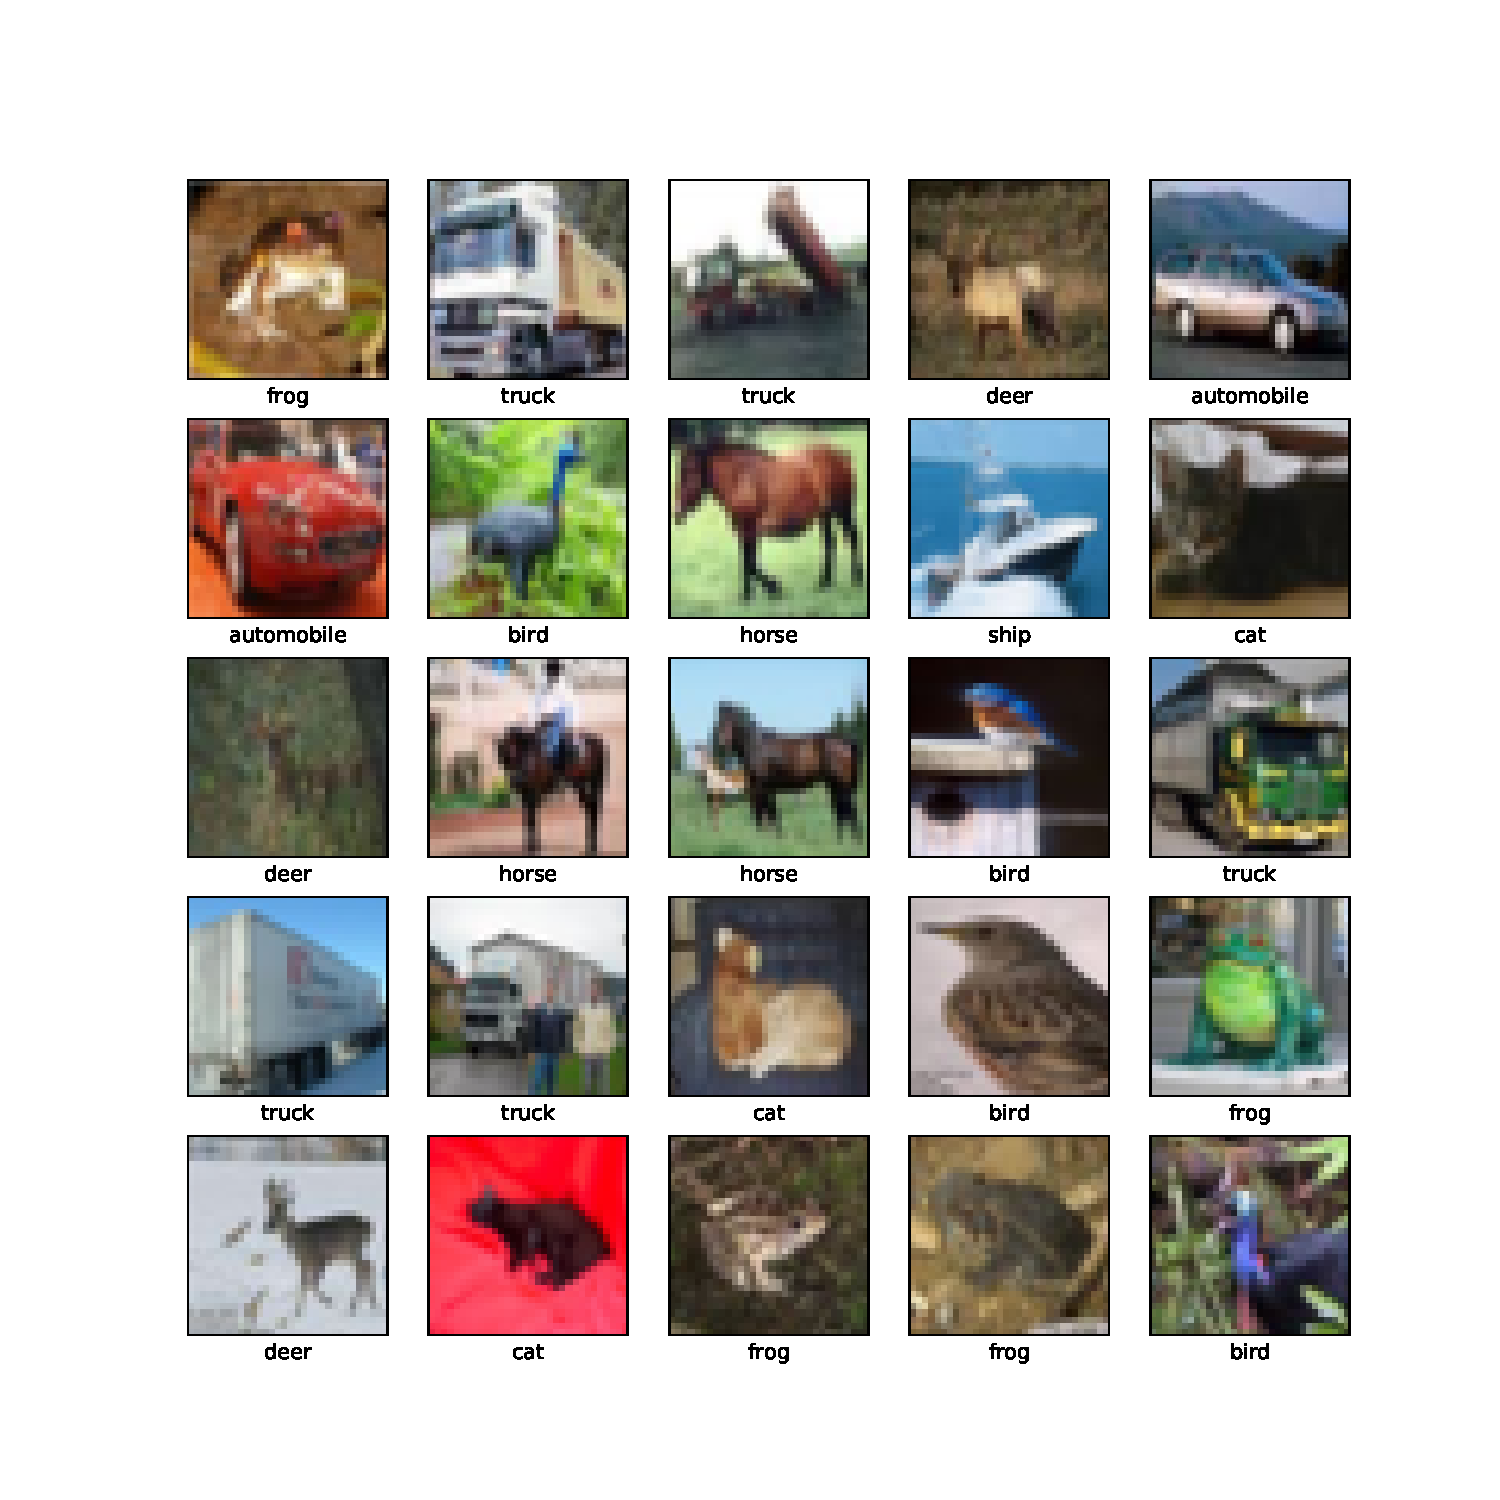
\includegraphics[trim = 25mm 145mm 25mm 15mm, clip, width=\textwidth]{CUDA/cifar-sample.pdf}
	\caption{Auszug von zehn Abbildungen des Datensatz \ac{cifar}-10}
	\label{fig:cifar-example}
\end{figure}

Um den Datensatz in die Python-Umgebung zu importieren, wird hier auf das Modul \python{keras.datasets} zurückgegriffen. Dies beinhaltet eine direkte Schnittstelle zum Datensatz \ac{cifar}-10, welcher durch den Aufruf der Funktion \PYTHON{load\_data()} auf das lokale System heruntergeladen wird. Im Hintergrund wird der Datensatz als gepackte Datei mit der Endung \mytt{.tar.gz} heruntergeladen und im Ordner \FILE{C:\textbackslash Users\textbackslash <Nutzername>\textbackslash .keras\textbackslash datasets} abgelegt. Nach dem Entpacken ist der Datensatz in mehreren serialisierten Objekten enthalten, welche über \PYTHON{pickle} in die Python-Umgebung geladen werden. Daraufhin kann auf die Trainingsdaten, Trainingslabel, Testdaten, und Testlabel über entsprechende Listen zugegriffen werden (\cref{src:cifarimport}). Um bei dem späteren Training das Vanishing-Gradient-Problem zu reduzieren \cite{Ide:2017}, werden die im Datensatz abgelegten RGB-Farbwerte mit dem Wertebereich von 9 bis 255 in Werte von 0 bis 1 umgerechnet. Das Listing~\ref{src:cifarimport} zeigt das Laden und Normalisieren der Daten.


\begin{code}
\begin{lstlisting}[language=MyPython, numbers=left,label={src:cifarimport}]
	(TRAIN_IMAGES, TRAIN_LABELS), (TEST_IMAGES, TEST_LABELS) =  datasets.cifar10.load_data()
	TRAIN_IMAGES = TRAIN_IMAGES / 255.0
	TEST_IMAGES  = TEST_IMAGES / 255.0
\end{lstlisting}
  \caption{Laden und Normalisieren des Datensatzes \ac{cifar}-10}
\end{code}


\subsubsection{Datensatz \ac{cifar}-100}\label{sec:dataset}


Der Datensatz \ac{cifar}-100 hingegen enthält zwar ebenfalls 60.000 Bilder, jedoch unterteilt in 100 Kategorien mit je 600 Bildern. Dabei gibt es zusätzlich 20 Oberkategorien, denen jeweils fünf der 100 Kategorien zugeordnet sind; siehe Tabelle~\ref{TabCIF100}.

\begin{figure}
    \begin{tabular} {l l} 
        \hline
        Superclass &	Classes\\
        \hline
        aquatic mammals & 	beaver, dolphin, otter, seal, whale\\
        fish & 	aquarium fish, flatfish, ray, shark, trout\\
        flowers & 	orchids, poppies, roses, sunflowers, tulips\\
        food containers &	bottles, bowls, cans, cups, plates\\
        fruit and vegetables &	apples, mushrooms, oranges, pears, sweet peppers\\
        household electrical devices &	clock, computer keyboard, lamp, telephone, television\\
        household furniture &	bed, chair, couch, table, wardrobe\\
        insects &	bee, beetle, butterfly, caterpillar, cockroach\\
        large carnivores &	bear, leopard, lion, tiger, wolf\\
        large man-made outdoor things &	bridge, castle, house, road, skyscraper\\
        large natural outdoor scenes &	cloud, forest, mountain, plain, sea\\
        large omnivores and herbivores &	camel, cattle, chimpanzee, elephant, kangaroo\\
        medium-sized mammals &	fox, porcupine, possum, raccoon, skunk\\
        non-insect invertebrates &	crab, lobster, snail, spider, worm\\
        people &	baby, boy, girl, man, woman\\
        reptiles &	crocodile, dinosaur, lizard, snake, turtle\\
        small mammals &	hamster, mouse, rabbit, shrew, squirrel\\
        trees &	maple, oak, palm, pine, willow\\
        vehicles 1 &	bicycle, bus, motorcycle, pickup truck, train\\
        vehicles 2 &	lawn-mower, rocket, streetcar, tank, tractor\\
    \end{tabular}
    \caption{Oberkategorien und Kategorien in \ac{cifar}-100 mit den Originalbezeichnungen}
    \label{TabCIF100}
    
\end{figure}


Der Datensatz kann ebenfalls heruntergeladen und direkt über Keras in TensorFlow importiert werden \cite{kaggle.21.09.2020}:

\begin{code}
    
\begin{lstlisting}[language=MyPython, numbers=left,label={src:cifarimport}]
    import tensorflow as tf
    from tensorflow.keras import datasets
    
    (TRAIN_IMAGES100, TRAIN_LABELS100), (TEST_IMAGES100, TEST_LABELS100) = tf.keras.datasets.cifar100.load_data()
	TRAIN_IMAGES100 = TRAIN_IMAGES100 / 255.0
    TEST_IMAGES100  = TEST_IMAGES100 / 255.0
    
\end{lstlisting}
  \caption{Laden und Normalisieren des Datensatzes \ac{cifar}-100}
\end{code}



%%%%%%
%
% $Autor: Wings $
% $Datum: 2021-05-14 $
% $Pfad: GitLab/Bilderkennung/Projects $
% $Dateiname: iris
% $Version: 4620 $
%
%%%%%%

%todo Manche Texte finden sich in TensorFlow.tex wieder. Dies ist zu ändern.
%Quelle: https://riptutorial.com/de/scikit-learn/example/6801/beispieldatensatze


\subsection{Datensatz Fisher's Iris Data Set}

Die Erkennung der Iris ist ein weiterer Klassiker zur Bildklassifizierung. Auch zu diesem Klassiker gibt es mehrere Tutorials. Der Datensatz Fisher's Iris Data Set\index{Datensatz!Fisher's Iris Data Set} wurde in R.A.~Fishers klassischer Arbeit von 1936 verwendet und kann im UCI Machine Learning Repository \index{UCI Machine Learning Repository} gefunden werden. \cite{Fisher:1936,Iris:2021,Schutten:2016} Es wurde vier Merkmale der Blumen Iris Setosa, Iris Versicolour und Iris Virginica vermessen. Für jede der drei Klassen stehen 50 Datensätze mit vier Attributen zur Verfügung. Gemessen wurden dabei jeweils die Breite und die Länge des Kelchblatts (Sepalum) sowie des Kronblatts (Petalum) in Zentimeter. \cite{Anderson:1935,Sahni:2006}. Eine Blumenart ist linear von den anderen beiden trennbar, aber die anderen beiden sind nicht linear voneinander trennbar.


Auf den Datensatz kann an mehreren Stellen zugriffen werden:

\begin{itemize}
    \item \href{https://archive.ics.uci.edu/ml/datasets/iris}{Archiv von Datensätzen für das Maschinelle Lernen der Univerität von Kalifornieren in Irvine} \cite{UCIIris:2021}
    \item \href{https://scikit-learn.org/stable/auto_examples/datasets/plot_iris_dataset.html}{Python Paket \FILE{skikitlearn}} \cite{scikit-learn:2011}
    \item \href{https://www.kaggle.com/uciml/iris}{Kaggle - Website für Maschinelles Lernen} \cite{KaggleIris:2018}
    %\item \url{https://gist.github.com/curran/a08a1080b88344b0c8a7}
\end{itemize}

Den Datensatz steht auf verschiedenen Webseiten zur Verfügung, allerdings muss auf den Aufbau des Datensatzes geachtet werden. Da es sich um eine Datei im Format CSV handelt, ist der Aufbau spaltenorientiert. In der Regel ist in der ersten Zeile der Titel der einzelnen Spalte angegeben: \texttt{sepal\_length}, \texttt{sepal\_width}, \texttt{petal\_length}, \texttt{petal\_width} und \texttt{species}. Die Werte sind in Zentimeter angegeben, die Spezie ist mit \texttt{setosa} für Iris Setosa, \texttt{versicolor} für Iris Versicolor und \texttt{virginica} für die Spezie Iris Virginica angegeben.
Die Spalten in diesem Datensatz sind:

\begin{itemize}
  \item Laufende Nummer
  \item Länge des  Kelchblatts (Sepal) in Zentimeter
  \item Breite des  Kelchblatts (Sepal) in Zentimeter
  \item Länge des Blütenblatts (Petal) in Zentimeter
  \item Breite des Blütenblatts (Petal) in Zentimeter
  \item Art    
\end{itemize}




Das Ziel ist die Klassifizierung der drei verschiedenen Iris-Arten anhand der Länge und Breite von Kelchblatt und Blütenblatt. Da der Datensatz mit der Bibliothek \PYTHON{sklearn} ausgeliefert wird, wird dieser Zugang gewählt. 

\begin{code}
  \begin{lstlisting}[language=MyPython, numbers=left,label={src:irisimport}]
from sklearn.datasets import load_iris
iris = load_iris()
  \end{lstlisting}
  \caption{Laden des Datensatzes Fisher's Iris Data Set\index{Datensatz!Fisher's Iris Data Set}}
\end{code}


Der Datensatz ist ein \PYTHON{dictionary}. Seine Schlüssel kann man sich leicht anzeigen lassen:

\begin{lstlisting}[language=MyPython, numbers=left]
>>> iris.keys()
\end{lstlisting}

Die zugehörige Ausgabe ist wie folgt:

\begin{lstlisting}[numbers=none]
    dict\_keys(['data', 'target', 'frame', 'target\_names', 'DESCR', 'feature\_names', 'filename'])
\end{lstlisting}



Die einzelnen Elemente kann man sich nun ansehen. Nach Eingabe des Befehls 

\begin{lstlisting}[language=MyPython, numbers=left]
iris['DESCR']
\end{lstlisting}

wird eine ausführliche Beschreibung ausgegeben:

\begin{code}
\begin{lstlisting}[language=MyPython, numbers=left]
'.. _iris_dataset:
    
Iris plants dataset
--------------------
    
**Data Set Characteristics:**
    
:Number of Instances: 150 (50 in each of three classes)
:Number of Attributes: 4 numeric, predictive attributes and the class
:Attribute Information:
   - sepal length in cm
   - sepal width in cm
   - petal length in cm
   - petal width in cm
   - class:
       - Iris-Setosa
       - Iris-Versicolour
       - Iris-Virginica
      
   :Summary Statistics:
   
   ============== ==== ==== ======= ===== ====================
   Min  Max   Mean    SD   Class Correlation
   ============== ==== ==== ======= ===== ====================
   epal length:    4.3  7.9   5.84   0.83    0.7826
   sepal width:    2.0  4.4   3.05   0.43   -0.4194
   petal length:   1.0  6.9   3.76   1.76    0.9490  (high!)
   petal width:    0.1  2.5   1.20   0.76    0.9565  (high!)
   ============== ==== ==== ======= ===== ====================
   
   :Missing Attribute Values: None
   :Class Distribution: 33.3% for each of 3 classes.
   :Creator: R.A. Fisher
   :Donor: Michael Marshall (MARSHALL%PLU@io.arc.nasa.gov)
   :Date: July, 1988
   
   The famous Iris database, first used by Sir R.A. Fisher. The dataset is taken
   from Fisher\'s paper. Note that it\'s the same as in R, but not as in the UCI\nMachine Learning Repository, which has two wrong data points.
   
   This is perhaps the best known database to be found in the
   pattern recognition literature.  Fisher\'s paper is a classic in the field and
   is referenced frequently to this day.  (See Duda & Hart, for example.)  The
   data set contains 3 classes of 50 instances each, where each class refers to a\ntype of iris plant.  One class is linearly separable from the other 2; the\nlatter are NOT linearly separable from each other.
   
   .. topic:: References
   
   - Fisher, R.A. "The use of multiple measurements in taxonomic problems"
     Annual Eugenics, 7, Part II, 179-188 (1936); also in "Contributions to
     Mathematical Statistics" (John Wiley, NY, 1950).
   - Duda, R.O., & Hart, P.E. (1973) Pattern Classification and Scene Analysis.
     (Q327.D83) John Wiley & Sons.  ISBN 0-471-22361-1.  See page 218.
   - Dasarathy, B.V. (1980) "Nosing Around the Neighborhood: A New System
     Structure and Classification Rule for Recognition in Partially Exposed
     Environments".  IEEE Transactions on Pattern Analysis and Machine
     Intelligence, Vol. PAMI-2, No. 1, 67-71.
   - Gates, G.W. (1972) "The Reduced Nearest Neighbor Rule".  IEEE Transactions
     on Information Theory, May 1972, 431-433.
   - See also: 1988 MLC Proceedings, 54-64.  Cheeseman et al"s AUTOCLASS II
     conceptual clustering system finds 3 classes in the data.
   - Many, many more ...'
\end{lstlisting}
\caption{Beschreibung des Datensatzes Fisher's Iris Data Set\index{Datensatz!Fisher's Iris Data Set}}
\end{code}

Mit der Eingabe

\begin{lstlisting}[language=MyPython, numbers=left]
    iris['feature_names']
\end{lstlisting}

erhält man die Namen der Attribute:

\begin{lstlisting}[numbers=none]
    ['sepal length (cm)',
    'sepal width (cm)',
    'petal length (cm)',
    'petal width (cm)']
\end{lstlisting}

Die Namen der Blumen, die nach der Eingabe

\begin{lstlisting}[language=MyPython, numbers=left]
    iris['target_names']
\end{lstlisting}

angezeigt werden, sind

\begin{lstlisting}[numbers=none]
    array(['setosa', 'versicolor', 'virginica'], dtype='<U10')
\end{lstlisting}

Zur weiteren Untersuchung werden die Daten mit den Überschriften in einen Datenrahmen aufgenommen.

\begin{lstlisting}[language=MyPython, numbers=left]
    X = pd.DataFrame(data = iris.data, columns = iris.feature_names)
    print(X.head())
\end{lstlisting}

Der Befehl \PYTHON{(X.head())} zeigt -- wie in Abbildung~\ref{TensorFlowHead} -- den Kopf des Datenrahmens an. Ersichtlich ist, dass jeder Datensatz aus vier Werten besteht. 

\begin{figure}[H]
    \GRAPHICSC{0.6}{1.0}{TensorFlow/IrisHead}
    \caption{Kopfzeilen des Datensatzes Fisher's Iris Data Set\index{Datensatz!Fisher's Iris Data Set}}\label{TensorFlowHead}
\end{figure}

Jeder Datensatz enthält auch schon in dem Schlüssel \PYTHON{target} seine Klassifikation. In der Abbildung~\ref{TensorFlowHeadType} ist dies für die ersten Datensätze aufgeführt.

\begin{lstlisting}[language=MyPython, numbers=left]
    y = pd.DataFrame(data=iris.target, columns = ['irisType'])
    y.head()
\end{lstlisting}

\begin{figure}[H]
    \GRAPHICSC{1.0}{1.0}{TensorFlow/IrisHeadType}
    \caption{Ausgabe der Kategorien des Datensatzes Fisher's Iris Data Set\index{Datensatz!Fisher's Iris Data Set}}\label{TensorFlowHeadType}
\end{figure}

Mittels des Befehls 

\begin{lstlisting}[language=MyPython, numbers=left]
    y.irisType.value_counts()
\end{lstlisting}

kann ermittel werden, wie viele Klassen vorliegen. Die Ausgabe des Befehls wird in der Abbildung~\ref{TensorFlowIrisTypes}
gezeigt; es ergeben sich 3 Klassen mit den Nummern $0$, $1$ und $2$. Jeweils 50 Datensätze sind ihnen zugeordnet.

\begin{figure}[H]
    \GRAPHICSC{1.0}{1.0}{TensorFlow/IrisTypes}
    \caption{Namen der Kategorien im Datensatz Fisher's Iris Data Set\index{Datensatz!Fisher's Iris Data Set}}\label{TensorFlowIrisTypes}
\end{figure}


%%%%%%
%
% $Autor: Wings $
% $Datum: 2021-05-14 $
% $Pfad: GitLab/Bilderkennung/Projects/Inahlt/General $
% $Dateiname: coco
% $Version: 4620 $
%
%%%%%%


\subsection{Common Objects in Context - COCO}


Der Datensatz \ac{coco} ist beschriftet und liefert Daten zum Trainieren von überwachten Computer-Vision-Modellen, die in der Lage sind, gemeinsamen Objekte im Datensatz zu identifizieren. Natürlich sind diese Modelle noch weit davon entfernt, perfekt zu sein. Daher bietet der Datensatz \ac{coco} einen Maßstab für die Bewertung der periodischen Verbesserung dieser Modelle durch die Computer-Vision-Forschung.\cite{Lin:2014,Coco:2021}

\bigskip

\begin{itemize}
    \item Objekterkennung
     \begin{itemize}
       \item Der Datensatz \ac{coco} enthält $\approx$ 330.000 Bilder.
       \item Der Datensatz \ac{coco} enthält $\approx$ 1.500.000 Annotationen für Objekte.
       \item Der Datensatz \ac{coco} enthält 80 Kategorien.
       \item Die Bilder haben jeweils fünf Überschriften.
       \item Die Bilder haben eine mittlere Auflösung  $640 \times 480$ Pixel.
     \end{itemize}  
  \item Semantische Segmentierung
    \begin{itemize}
        \item Panoptische Segmentierung erfordert Modelle zum Ziehen von Grenzen zwischen Objekten bei der semantischen Segmentierung.
    \end{itemize}

  \item Erkennung von Schlüsseln
    \begin{itemize}
      \item Die Bilder enthalten 250.000 Personen, die mit den entsprechenden Schlüssel  beschriftet sind.
    \end{itemize}
\end{itemize}




Aufgrund der Größe und der häufigen Verwendung des Datensatzes gibt es zahlreiche Werkzeuge, zum Beispiel COCO-annotator und COCOapi, um auf die Daten zuzugreifen.


Eigentlich besteht der Datensatz \ac{coco} aus mehreren, die jeweils für eine bestimmte Aufgabe des Maschinellen Lernens gemacht wurden. Die erste Aufgabe ist die Bestimmung von umgebenden Rechtecke für Objekte. Das heißt, es werden Objekte identifiziert und die Koordinaten des umgebenden Rechtecke ermittelt. Die erweiterte Aufgabe ist die Objektsegmentierung. Hierbei werden auch Objekte identifiziert, aber zusätzlich anstelle der umgebenden Rechtecke Polygonzüge, die die Objekte eingrenzen. Die dritte klassische Aufgabe ist die Stoffsegmentierung. Das Modell soll eine Objektsegmentierung durchführen, aber nicht auf einzelnen Objekten, sondern auf kontinuierlichen Hintergrundmustern wie Gras oder Himmel.


\bigskip

Die Annotationen sind im Format JSON hinterlegt. Das Format JSON ist ein Wörterbuch mit Schlüssel-Wert-Paare in geschweiften Klammern. Es kann auch Listen, geordnete Sammlungen von Elementen innerhalb von geschweiften Klammern, oder Wörterbücher enthalten, die darin verschachtelt sind.

\begin{code}
\begin{lstlisting}[language=python]
{
  "info": {...},
  "licenses": {...},
  "images": {...},
  "categories": {...},
  "annotations": {...}
}    
\end{lstlisting}
\caption{Informationen des Datensatzes \ac{coco}}
\end{code}



“info” section

Das Wörterbuch zum Abschnitt \PYTHON{info} enthält Metadaten über den Datensatz. Für den offiziellen Datensatz \ac{coco} sind es folgende Informatinen:


\begin{code}
\begin{lstlisting}[language=python]
{
    "description": "COCO 2017 Dataset",
    "url": "http://cocodataset.org",
    "version": "1.0",
    "year": 2017,
    "contributor": "COCO Consortium",
    "date_created": "2017/09/01"
}
\end{lstlisting}
\caption{Metainformationen des Datensatzes \ac{coco}}
\end{code}

Wie man sieht, sind nur grundlegende Informationen enthalten, wobei der Wert url auf die offizielle Website des Datensatzes verweist. Dies ist bei Datensätzen für Maschinelles Lernen üblich, um auf ihre Websites für zusätzliche Informationen zu verweisen. Dort kann man zum Beispiel Informationen wie und wann die Daten erfasst wurden.

\bigskip


Im Abschnitt licenses finden Sie Links zu Lizenzen für Bilder im Datensatz mit der folgenden Struktur:

\begin{code}
\begin{lstlisting}[language=python]
[
{
    "url": "http://creativecommons.org/licenses/by-nc-sa/2.0/", 
    "id": 1, 
    "name": "Attribution-NonCommercial-ShareAlike License"
},
{
    "url": "http://creativecommons.org/licenses/by-nc/2.0/", 
    "id": 2, 
    "name": "Attribution-NonCommercial License"
},
...
]
\end{lstlisting}
\caption{Lizenzinformationen des Datensatzes \ac{coco}}
\end{code}

\bigskip


\bigskip

Dieses Wörterbuch images ist wohl das zweitwichtigste und enthält Metadaten über die Bilder.

Das Wörterbuch images enthält das Feld id. In diesem Feld wird die Lizenz des Bildes angegeben. Der vollständige Text ist in der URL angegeben. Bei der Verwendung der Bilder ist sicherzustellen, dass keine Lizenzverletzung erfolgt. Im Zweifel sollte auf die Verwendung verzichtet werden. Das heißt aber auch, dass man bei der Erstellung eines eigenen Datensatzes jedem Bild eine entsprechende Lizenz zuweist. 


\begin{code}
\begin{lstlisting}[language=python]
{
    "license": 3,
    "file_name": "000000391895.jpg",
    "coco_url": "http://images.cocodataset.org/train2017/000000391895.jpg",
    "height": 360,
    "width": 640,
    "date_captured": "2013-11-14 11:18:45",
    "flickr_url": "http://farm9.staticflickr.com/8186/8119368305_4e622c8349_z.jpg",
    "id": 391895
}
\end{lstlisting}
\caption{Bildinformationen des Datensatzes \ac{coco}}
\end{code}


Das wichtigste Feld ist das Feld id. Dies ist die Nummer, die in im Abschnitt annotations verwendet wird, um das Bild zu identifizieren. Wenn man also zum Beispiel die Anmerkungen für die gegebene Bilddatei identifizieren möchte, muss man den Wert des Felds id für das entsprechende Bilddokument in Abschnitt images überprüfen und dann in im Abschnitt annotations einen Querverweis darauf machen.

Im offiziellen Datensatz \ac{coco} ist der Wert des Feldes id der gleiche wie der Name \FILE{file\_name} nach Entfernen der führenden Nullen. Falls man einer benutzerdefinierte Datensatz \ac{coco} verwendet, muss dies nicht unbedingt der Fall sein. 

\bigskip

"Abschnitt "Kategorien

Der Abschnitt categories unterscheidet sich ein wenig von den anderen Abschnitten. Er ist für die Aufgabe der Objekterkennung und Segmentierung und für die Aufgabe der Stoffsegmentierung konzipiert.

Für die Objekterkennung und die Objektsegmentierung erhält man die Informationen gemäß des Lstings~\ref{cocoObject}

\begin{code}
    \begin{lstlisting}[language=python]
[
{"supercategory": "person", "id": 1, "name": "person"},
{"supercategory": "vehicle", "id": 2, "name": "bicycle"},
{"supercategory": "vehicle", "id": 3, "name": "car"},
...
{"supercategory": "indoor", "id": 90, "name": "toothbrush"}
]
\end{lstlisting}

\caption{Klasseninformationen des Datensatzes \ac{coco}}\label{cocoObject}
\end{code}

In dem Abschnitt enthalten die Listen die Kategorien von Objekten, die auf Bildern erkannt werden können. Jede Kategorie hat eine eindeutige Nummer id und sie sollte im Bereich [1, Anzahl der Kategorien] liegen. Kategorien werden auch in Oberkategorien gruppiert, die man in Programmen verwenden kann, um beispielsweise Fahrzeuge im Allgemeinen zu erkennen, wenn es Ihnen egal ist, ob es sich um ein Fahrrad, ein Auto oder einen LKW handelt.

\bigskip

Für die Stoffsegmentierung existieren eigene Listen, siehe Listing~\ref{cocoStuff}

\begin{code}
\begin{lstlisting}[language=python]
[
{"supercategory": "textile", "id": 92, "name": "banner"},
{"supercategory": "textile", "id": 93, "name": "blanket"},
...
{"supercategory": "other", "id": 183, "name": "other"}
]
\end{lstlisting}
\caption{Stoffinformationen des Datensatzes \ac{coco}}\label{cocoStuff}
\end{code}

Die Nummer der Kategorien in diesem Abschnitt beginnen hoch, um Konflikte mit der Objektsegmentierung zu vermeiden, da diese Aufgaben bei der panoptischen Segmentierungsaufgabe zusammen durchgeführt werden können. Die Werte von 92 bis 182 repräsentieren das wohldefiniertes  Hintergrundmaterial, während der Wert 183 alle anderen Hintergrundtexturen repräsentiert, die keine eigenen Klassen haben.

\bigskip

Der Abschnitt annotations ist der wichtigste Abschnitt des Datensatzes, der für jede Aufgabe wichtige Informationen für den spezifischen Datensatz enthält.

\begin{code}
    \begin{lstlisting}[language=python]
{
    "segmentation":
    [[
    239.97,
    260.24,
    222.04,
    ...
    ]],
    "area": 2765.1486500000005,
    "iscrowd": 0,
    "image_id": 558840,
    "bbox":
    [
    199.84,
    200.46,
    77.71,
    70.88
    ],
    "category_id": 58,
    "id": 156
}
\end{lstlisting}
\caption{Annotationen des Datensatzes \ac{coco}}\label{cocoAnnotation}
\end{code}

Die Felder gemäß Listing~\ref{cocoAnnotation} haben folgende Bedeutung.

\begin{description}
  \item["{}segmentation":] Dies ist eine Liste von Segmentierungsmasken für Pixel; dies ist eine abgeflachte Liste von Paaren, so dass man den ersten und den zweiten Wert (x und y im Bild) nehmen sollten, dann den dritten und den vierten usw., um Koordinaten zu erhalten; dabei ist zu beachten, dass dies keine Bildindizes sind, da es sich um Fließkommazahlen handelt --- sie werden von Tools wie COCO-annotator aus den Pixelkoordinaten erstellt und komprimiert.

  \item ["{}area":] Dies entspricht die  Anzahl der Pixel innerhalb einer Segmentierungsmaske.

  \item ["{}iscrowd":] Dies ist eine Fahne, die anzeigt, ob die Beschriftung für ein einzelnes Objekt (Wert 0) oder für mehrere nahe beieinander liegende Objekte (Wert 1) gilt; bei Füllungssegmentierung ist dieses Feld immer 0 und wird ignoriert.

  \item ["{}image\_id":] Das Feld id entspricht der Nummer des Feldes id vom Wörterbuch images; Warnung: dieser Wert sollte zum Querverweis des Bildes mit anderen Wörterbüchern verwendet werden, also nicht das Feld id.

  \item ["bbox":] In der Rubrik befinden sich die umgebenden Rechtecke beziehungsweise Bounding Box, das heißt, die Koordinaten in Form der x- und y-Koordinate der oberen, linken Ecke, sowie die Breite und die Höhe des Rechtecks um das Objekt; es ist sehr nützlich, um einzelne Objekte aus Bildern zu extrahieren, da dies in vielen Sprachen wie Python durch den Zugriff auf das Bild-Array erfolgen kann wie; 
  
  \PYTHON{cropped\_object = image[bbox[0]:bbox[0] + bbox[2], bbox[1]:bbox[1] + bbox[3]]}
  
  \item ["category\_id":] Das Feld enthält die Klasse des Objekts, entsprechend dem Feld id aus dem Abschnitt "categories"

  \item ["{}id":] Die Nummer ist der eindeutige Bezeichner für die Annotation; dabei ist beachten, dass dies nur die ID der Annotation ist, sie verweist also nicht auf das jeweilige Bild in anderen Wörterbüchern.

  \medskip
   
  Bei der Arbeit mit Crowd-Bildern ("iscrowd": 1) kann der Teil "Segmentierung" ein wenig anders sein:

  \begin{lstlisting}
"segmentation":
{
  "counts": [179,27,392,41,..,55,20],
  "size": [426,640]
}
  \end{lstlisting}

  \bigskip

  Dies liegt daran, dass bei einer großen Anzahl von Pixeln die explizite Auflistung aller Pixel, die eine Segmentierungsmaske erstellen, sehr viel Platz benötigen würde. Stattdessen verwendet der Datensatz \ac{coco} eine benutzerdefinierte Komprimierung \ac{rle}, die sehr effizient ist, da Segmentierungsmasken binär sind und \ac{rle} für ausschließlich Nullen und Einsen die Größe um ein Vielfaches verringern kann.

\end{description}


}

%%%%%%
%
% $Autor: Wings $
% $Datum: 2021-05-14 $
% $Pfad: GitLab/Bilderkennung/Projects/Inhalt/General $
% $Dateiname: ImageNet
% $Version: 4620 $
%
%%%%%%


\subsection{ImageNet}

ImageNet\index{Datensatz!ImageNet}\index{ImageNet!\see{Datensatz}} ist eine Bilddatenbank mit mehr als 14 Millionen Bildern, die permanent wächst. Jedes Bild wird einem Substantiv zugeordnet. Zu jeder Kategorie gibt es im Schnitt mehr als 500 Bilder. ImageNet enthält mehr als 20.000 Kategorien in englischer Sprache mit einer typischen Kategorie wie beispielsweise \glqq Ballon\grqq{} oder \glqq Erdbeere\grqq. Die Datenbank mit Anmerkungen zu Bild-URLs von Drittanbietern ist direkt über ImageNet frei zugänglich, obwohl die eigentlichen Bilder nicht im Besitz von ImageNet sind. \cite{Deng:2009,Shankar:2020,Krizhevsky:2012b}

%%%
%
% $Autor: Wings $
% $Datum: 2021-05-14 $
% $Pfad: GitLab/MLEdgeComputer/Inhalt/General $
% $Dateiname: VisualWakeWords 
% $Version: 4620 $
%
% !TeX spellcheck = de_DE
%
%%%



\subsection{Visual Wake Words}

Der Datensatz \glqq Visual Wake Words\grqq{}  besteht aus 115.000 Bildern, von denen jedes mit der Angabe versehen ist, ob es eine Person enthält oder nicht. \cite{Chowdhery:2019} %\url{https://arxiv.org/abs/1906.05721}
Aus dem Datensatz \ac{coco} werden Bilder extrahiert. Da der Datensatz \ac{coco} Informationen über die Bilder zur Verfügung stellt, kann bei der Extraktion abgefragt werden, ob innerhalb eines umgebenden Rechtecks sich eine Person befindet oder nicht. Die Daten werden mit der Information gekennzeichnet.










%\Ausblenden
{

%todo http://vis-www.cs.umass.edu/lfw/ Labeled Faces in the Wild \cite{Huang:2014}

\section{Modelle}

Bei der Installation des Projekts jetson-inference\index{jetson-inference} von NVidia bietet das Hilfsprogramm eine große Auswahl an vortrainierten Deep-Learning-Modellen zum Herunterladen an. Darunter befinden sich bekannte wie das AlexNet\index{AlexNet} von 2012 sowie verschiedene sogenannte \ac{resnets}. Ebenfalls dabei sind SSD-Mobilenet-V2\index{SSD-Mobilenet-V2}, das 90 Objekte vom Apfel bis zur  Zahnbürste erkennt, und DeepScene\index{DeepScene} der Universität Freiburg zur Erkennung von Objekten im Straßenverkehr. 

Um weitere Modelle herunterzuladen, kann der Model Downloader aufgerufen werden:

\medskip

\SHELL{\$ cd jetson-inference/tools} \newline 
\SHELL{\$ ./download-models.sh} 

\medskip

Die Modelle GoogleNet und ResNet-18, die auf der Bilddatenbank ImageNet\index{ImageNEt} beruhen, werden im Build-Schritt automatisch heruntergeladen. In der Tabelle~\ref{Database:TrainedModell} sind alle Modelle aufgelistet, die im Projekt jetson-inference zur Verfügung stehen. Die erste Spalte der Tabelle ist der Name der Struktur des Modells. \cite{Alom:2018}. In der zweiten Spalte ist der Übergabeparameter für das Argument \PYTHON{--network} des Programms \FILE{imagenet-camera.py} enthalten.

\medskip

\begin{table}
  \centering
  \begin{tabular}[h]{lcr}
    \textbf{Network}              & \textbf{CLI argument} & \textbf{NetworkType enum} \\ \hline
    AlexNet\index{AlexNet}        & alexnet               & ALEXNET \\
    GoogleNet\index{GoogleNet}    & googlenet             & GOOGLENET \\
    GoogleNet-12                  & googlenet-12          & GOOGLENET\_12 \\
    ResNet-18\index{ResNets}      & resnet-18             & RESNET\_18 \\
    ResNet-50                     & resnet-50             & RESNET\_50 \\
    ResNet-101                    & resnet-101            & RESNET\_101 \\
    ResNet-152                    & resnet-152            & RESNET\_152 \\
    VGG-16\index{VGG}             & vgg-16                & VGG-16 \\
    VGG-19                        & vgg-19                & VGG-19 \\
    Inception-v4\index{Inception} & inception-v4          & INCEPTION\_V4 \\
  \end{tabular}
  \caption{Vortrainierte Modelle des Projekts jetson-inference}\label{Database:TrainedModell}
\end{table}





%todo \input{../Inhalt/JetsonNano/MobileNet}

%todo %%%%%%
%
% $Autor: Wings $
% $Datum: 2021-05-14 $
% $Pfad: GitLab/MLEdgeComputer/ $
% $Dateiname: FaceNet
% $Version: 4620 $
%
%%%%%%

\section{FaceNet}

\cite{Schroff:2015}

%facenet-120\cite{Schroff:2015}

FaceNet lernt eine Abbildung von Gesichtsbildern auf einen kompakten euklidischen Raum, in dem Abstände direkt einem Maß für die Ähnlichkeit von Gesichtern entsprechen. Sobald dies geschehen ist, sind Aufgaben wie Gesichtserkennung, -verifizierung und -clusterung mit Standardtechniken (unter Verwendung der FaceNet-Einbettungen als Merkmale) einfach zu erledigen.
Verwendet ein Deep CNN, das trainiert wird, um die Einbettung selbst zu optimieren, anstatt die Ausgabe einer dazwischenliegenden Engpassschicht zu verwenden. Das Training erfolgt mit Triplets: ein Bild eines Gesichts ("Anker"), ein weiteres Bild desselben Gesichts ("positives Exemplar") und ein Bild eines anderen Gesichts ("negatives Exemplar"). Der Hauptvorteil liegt in der Repräsentationseffizienz: Mit nur 128 Byte pro Gesicht kann eine Spitzenleistung erzielt werden (Rekordgenauigkeit von 99,63 \% bei LFW, 95,12 \% bei Youtube Faces DB).

siehe \url{../../MLbib/CNN/class10_FaceNet.pdf}



FaceNet ist ein tiefes Faltungsneuronales Netzwerk, das von Google-Forschern entwickelt und um 2015 eingeführt wurde, um die Hürden bei der Gesichtserkennung und -verifizierung effektiv zu lösen. Der FaceNet-Algorithmus transformiert das Gesichtsbild in einen 128-dimensionalen euklidischen Raum, ähnlich wie beim Word Embedding[9]. Das so erstellte FaceNet-Modell wird auf Triplett-Verlust trainiert, um die Ähnlichkeiten und Unterschiede auf dem bereitgestellten Bilddatensatz zu erfassen. Die vom Modell erzeugten Einbettungen mit 128 Dimensionen können verwendet werden, um Gesichter auf sehr effektive und präzise Weise zu clustern. Durch die Verwendung von FaceNet-Embeddings als Merkmalsvektoren könnten nach der Erstellung des Vektorraums Funktionalitäten wie Gesichtserkennung und -verifikation implementiert werden[10]. Kurz gesagt, die Abstände für die ähnlichen Bilder würden viel näher sein als die zufälligen nicht ähnlichen Bilder. Die allgemeine Blockdarstellung des FaceNet-Ansatzes der Gesichtserkennung ist in Abb.1 dargestellt.

siehe \url{../../MLbib/CNN/10.1109ICACCS.2019.8728466.pdf}

Eingabeformat? Farben? Pixelauflösung?

%
%Detect-COCO-Airplane coco-airplain Flugzeuge
%Detect-COCO-Bottle coco-bottle Flaschen
%Detect-COCO-Chair coco-chair Stühle
%Detect-COCO-Dog coco-dogs Hunde
%ped-100 pednet Fußgänger
%multiped-500 multiped Fußgänger und Gepäck

%network=googlenet?
%ResNet-18

}
